%Paper to submit to PPSN IX

\documentclass{llncs}
%
\usepackage{makeidx}  % allows for indexgeneration
\usepackage[pdftex]{graphics}
\usepackage{graphicx}

%
\begin{document}

\title{Ecosystem Dynamics\\for Creative Image Generation}

\author{Andr\'ea Machizaud, Vincent Gardeux and Stefan Bornhofen}

\institute{Ecole Internationale des Sciences\\
du Traitement de l'Information\\
Avenue du Parc\\
95011 Cergy-Pontoise Cedex, France}

\maketitle

\begin{abstract}
Generative artists are constantly searching for new methods which innovate or enhance the esthetic value of their works. Over the last years, there has been a growing interest in using the swarm paradigm, i.e. in designing decentralized systems with mobile agents that collaborate on the creation of an emerging piece of art. In particular, "creative ecosystems" are conceived based on characteristic features of natural ecosystems, where organisms not only interact with one another and with their environment, but also complete an entire life cycle. The present paper [... bla bla... to be written as soon as we have the conlusion section].
\end{abstract}
%
\section{Introduction}

Generative art is one of the most fascinating blends between art and science. It covers any practice "where the artist uses a system, such as a set of natural language rules, a computer program, a machine, or other procedural invention, which is set into motion with some degree of autonomy contributing to or resulting in a completed work of art." \cite{Galanter2003}. The key feature in this approach is a generative system providing an automated method for artistic output. The output exhibits stylistic invariants, but also diverse and unpredictable facets, due to complex interactions between the system components and a number of involved parameters. The artistic value of the generated pieces can subsequently be assessed by the user. While the present paper focuses on the creation of images, generative art applies to many other forms including music, 3D sculpture or animation.

The artist typically guides the generative system via interactive evolution \cite{Takagi2001}, assigning fitness values to the pieces, and selecting which ones will survive and reproduce. Offspring is created using mutation and recombination rules, which give birth to a new generation of individuals. This process forms a cooperation between the human sense of esthetics and the technological means of the computer, allowing man and machine to conjointly work on art that "neither could easily produce alone" \cite{Sims1991}. Typical examples for this approach are images created by fractal algorithms \cite{Chapuis2001,Draves2005}, cellular automata \cite{Ashlock2009} and L-systems \cite{McCormack2004,Bornhofen2006}.

The use of swarm models has also been studied in this context \cite{Aupetit2003,Greenfield2005}. Inspired by the behavior of ants, artificial agents deposit colors on a canvas and follow simple rules of motion and reaction to the colors they encounter, just like natural ants move and react to pheromones, collaboratively working on an emerging piece of art. However, these agents do not possess other life-like features such as growth, metabolism or reproduction.

More recently, it has been suggested to explore the application of ecosystem dynamics for the creation of works of generative art \cite{McCormack2007,Dorin2008}. In these models, termed "creative ecosystems", the agents not only interact with one another and with their environment, but also complete a life cycle, reproduce and potentially evolve. The approach raises a number of interesting questions about which ecosystem mechanisms are most useful for creative design, how they can be adapted to generative art, and what their contribution on the work of art can be. As one of the pioneering results in this field, it has been shown that niche construction can considerably increase the diversity and the heterogeneity of artistic output \cite{McCormack2009,McCormack2010}.

The present paper extends this approach by modeling a generative ecosystem with resource consumption and predator-prey relationships, and by evaluating their impact on the produced images. We argue that the introduction of an energy budget to the agent model not only allows the user to partially control the creation process, but also to enrich the overall visual experience, by mapping the energy level of the agents to artistic dimensions such as line width or color.

The rest of the paper is organized as follows. In the next section, the ecosystem model is briefly presented. Several experiments of image generation are described in section three. Section four concludes the paper and discusses the perspectives on the approach.

\section{Model description}
%
The presented model is inspired from existing studies on swarm based generative art: artificial agents move, reproduce and evolve in a two-dimensional continuous environment, leaving a trail as they roam around. The environment can be considered as a canvas, and the trails are lines that progressively compose an image. The image is complete when there are no more agents in the environment \cite{Annunziato,McCormack2010}.

As a complement to the previous works, we introduce a simplified energy management and explore its potential for esthetic image generation. In particular, we focus on the following dynamics: food ingestion, predatory behavior and agent coloration. In the two above cited works, an agent dies when it crosses an existing trail. This constraint has been lifted and replaced by death through predation and starvation, i.e. total energy loss.

\subsection{Phenotype}

The current state of an agent is described by
\begin{itemize}
\item \textit{location}, \textit{speed}, \textit{orientation}: spatial information. In the scope of this paper, \textit{speed} is a constant value;
\item \textit{energy}: a positive real number denoting the energy budget which is cunsumed by movements. The energy level can be increased by absorbing resources from the environment. If it falls below zero, the agent dies;
\item \textit{covColor}: a covering color which changes according to the colors of the ingested ressources. The overall agent color is a blend between the covering color and the (genotypic) priming color (see below).
\end{itemize}

\subsection{Genotype}

In addition to the phenotypic information which varies over time, the agent behavior is ruled by a set of constant genetic characteristics. At reproduction, the offspring inherits these values some of which, depending on the simulation setup, may be affetced by random mutations.

\begin{itemize}
\item \textit{curvature}: the basic rate of curvature of the agent movement. A curvature of zero signifies a straight line;
\item \textit{irrationality}: the degree of variation superposed to the basic curvature. The higher this value, the more chaotic the movement, producing less predictable patterns;
\item \textit{fecundity}: the probability of producing a child agent per time step;
\item \textit{mortality}: the probability of dying per time step;
\item \textit{offset}: the offset angle of the children that separate form the parent agent;
\item \textit{divRatio}: the proportion of energy an agent allocates to its child at reproduction;
\item \textit{sensorRange}: the range of perception in the environment. An agent senses resources and other agents within this distance;
\item \textit{ingRange}: the maximum distance which allows ingesting food from the environment;
\item \textit{consumption}: the amount of consumed energy per covered distance;
\item \textit{agility}: the capacity to rapidly orient towards a target location when grazing, hunting or fleeing. The higher this value, the smaller the executed turning radius;
\item \textit{prColor}: the underlying priming color of the agent;
\item \textit{prStrength}: the relative strength of the priming color versus the covering color.
\end{itemize}

\subsection{Hunting and feeding}

We defined two types of agents: grazers and predators. Both exhibit the same basic moving behavior as long as no objects exist within their perception range. Grazing agents are attracted by static food bits which are placed in the environment. These food bits possess a certain amount of energy (\textit{resEnergy}) as well as a color (\textit{resColor}) which acts on the agent covering color. Predators hunt grazers but not static resources. When grazers sense predators, they start to flee in the opposite direction even if they have previously been heading for food bits. As soon as a chased entity enters the ingestion range, the agent increases its energy level by that of the target.

\subsection{Coloration}

When an agent feeds from the environment, its covering color updates according to the color and energy of the ingested resource:

\begin{displaymath}
covColor = \frac{covColor * energy + resColor * resEnergy}{energy + resEnergy}
\end{displaymath}

The trails are colored after the current overall color of the agents, called "complexion", which is a weighted mean of primary and covering color: the higher the energy level, the higher the influence of the covering color.

\begin{displaymath}
complexion = \frac{prColor * prStrength + covColor * energy}{prStrength + energy}
\label{Equation:Complexion}
\end{displaymath}

\section{Experiments}

\subsection{Guided ecosystem art}

The "resources consumption" component of the model may be used to drive the agents during the production of the image. Each grazing agent has a basic behaviour if no resource is in its detection range, but it will be attracted by nearby resources. They will so follow the resources and die when no more resource can be found. In order to illustrate the emerging behaviour of these rules, one simulate a grazing agent and several resources drops in the ecosystem (cf Figure \ref{Picture:Basic})
\begin{figure}[!ht]
\centering
\includegraphics[scale=.2]{Basic.jpg}
\label{Picture:Basic}
\caption{Resulting picture of an ecosystem art driven by resources}
\end{figure}
We can see that the agent follows the resources trail. The resulting picture will greatly depends on the initialization of the resource drops.

In order to test this behaviour in more complex resources disposion, one initialize resources following the "ICSI" letters. After that, one agent have been initialized on the bottom of each letter. The following picture (cf Figure \ref{Picture:ICSI}) shows the resulting picture.
\begin{figure}[!ht]
\centering
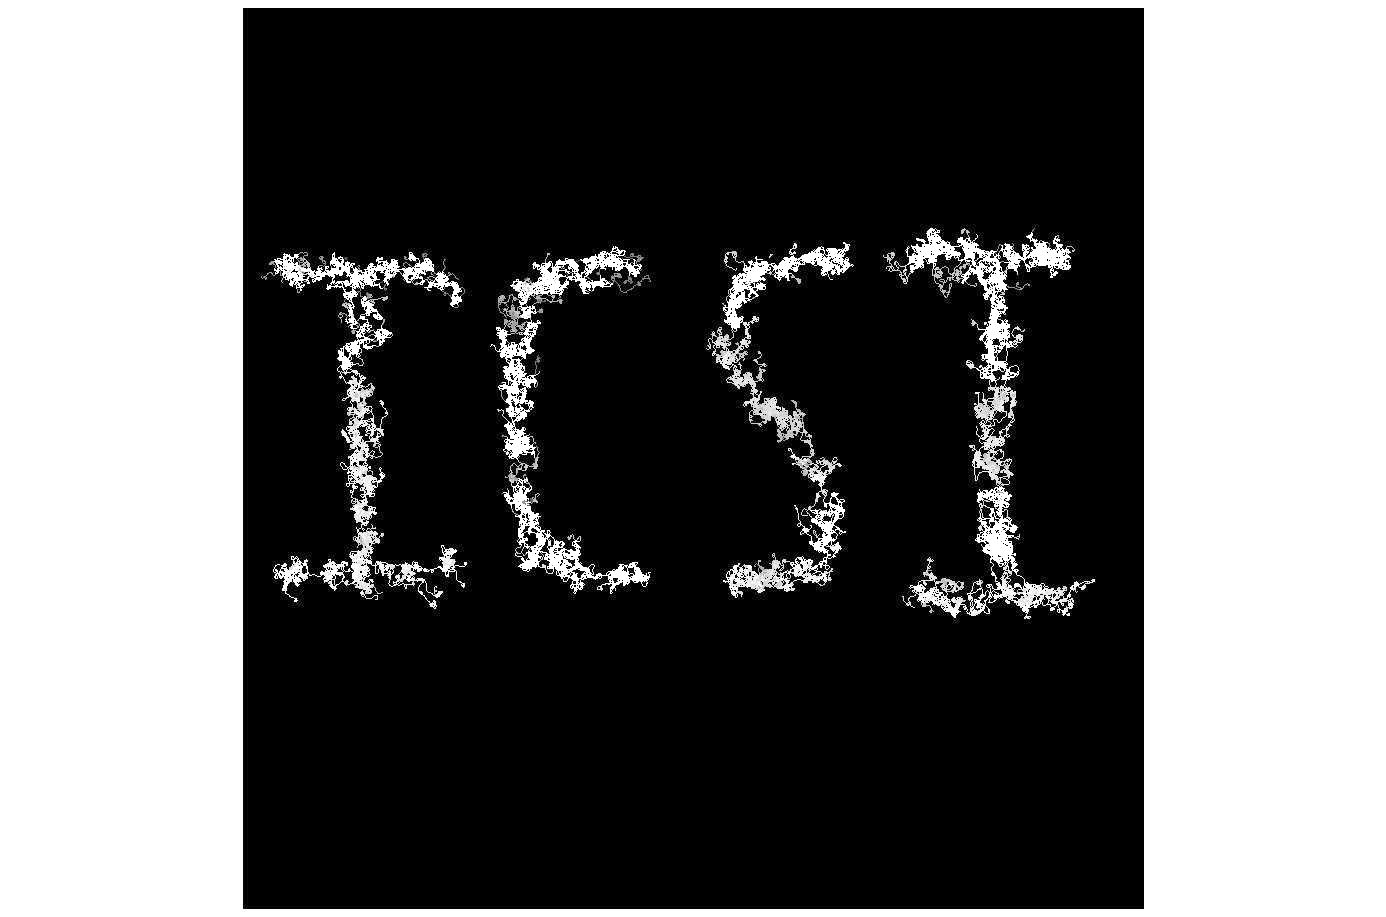
\includegraphics[scale=.2]{ICSI2G.jpg}
\label{Picture:ICSI}
\caption{Resulting picture of an ecosystem art driven by resources}
\end{figure}
We can see that each agent follows the letter on which it has been disposed. The image production is partly guided by the original disposition of the resources on the canvas. The other movements are generated by the irrationality parameter (high in the previous picture, leading to a chaotic movement, but still along the resources drops).

An interesting extension of this behaviour is to use an image in order to initialize the resource drops on the canvas. Indeed, the canvas can be assimiled to a grid in which each compartment have a $(x,y)$ position. A food bit will be deposed in the grid, corresponding to the $(x,y)$ pixel in the image. The agents will so follow the resources drops in the ecosystems and their color will evolve following the complexion equation \ref{Equation:Complexion}. The agents will "redraw" the initial picture, depending on its behaviour (cf Figure \ref{Picture:Image}).
\begin{figure}[!ht]
\centering

\includegraphics[scale=.4]{toto.jpg}
\label{Picture:Image}
\caption{Resulting picture of an ecosystem art driven by resources}
\end{figure}
We can see that its sooooo beautiful, I could die watching this!

\section{Discussion}




\section{Conclusion}

\begin{thebibliography}{5}
%
\bibitem{Galanter2003} Galanter, P., What is Generative Art? Complexity Theory as a Context for Art Theory, in
International Conference on Generative Art. 2003: Milan, Italy.
\bibitem{Peitgen2005} Peitgen PO, Richter PH. The beauty of fractals: images of complex dynamic systems. New York: Springer; 1986.
\bibitem{Burraston2005} Burraston, D. and Edmonds, E. (2005) Cellular Automata in Generative Electronic Music and Sonic Art : A Historical and Technical Review. Digital Creativity 16(3) pp. 165-185
\bibitem{Bonabeau1999} E. Bonabeau, M. Dorigo, and G. Theraulaz, Swarm intelligence: from natural to artificial systems, Oxford University Press, 1999
\bibitem{Aupetit2003} S\'ebastien Aupetit, Vincent Bordeau, Nicolas Monmarch�, Mohamed Slimane, and Gilles Venturini. Interactive Evolution of Ant Paintings. In IEEE Congress on Evolutionary Computation, volume 2, pages 1376-1383, Canberra, 8-12 december 2003. IEEE Press
\bibitem{Greenfield2005} Greenfield, G., Evolutionary methods for ant colony paintings, Applications of Evolutionary Computing, EvoWorkshops 2005 Proceedings, Springer-Verlag Lecture Notes in Computer Science, LNCS 3449 (eds. F. Rotlauf et al.), 2005, 478-487.
\bibitem{Takagi2001} H. Takagi. Interactive evolutionary computation: fusion of the capabilities of EC optimization and human evaluation. In Proceedings of the IEEE, volume 89, pages 1275-1296, September 2001.
\bibitem{Chapuis2001} Chapuis, J. and Lutton, E. (2001). ArtiE-Fract : Interactive evolution of fractals. In Proceedings of the 4th International Conference on Generative Art, Milan, Italy, pages 12-14.
\bibitem{Kwong2004} H. Kwong and C.Jacob. Evolutionary exploration of dynamic swarm behaviour. IEEE Congress on Evolutionary Computation, 2003.
\bibitem{Boyd2004} J. E. Boyd, G. Hushlak, C. Jacob, P. Nuytten, M. Sayles, SwarmArt: Interactive Art from Swarm Intelligence, in proceedings of ACM Multimedia 2004, October 12-14, 2004, New York, NY.
\bibitem{Ashlock2009} D. Ashlock and J. Tsang, Evolved Art via Control of Cellular Automata in Proceedings of the 2009 Congress on Evolutionary Computation, PP 3338-3344, 2009.
\bibitem{Sims1991} Sims, K. (1991). Artificial evolution for computer graphics. Computer Graphics, 25(4):319-328.
\bibitem{McCormack2004} McCormack, J. 2004, Aesthetic Evolution of L-Systems Revisited, in Raidl, G.R., S. Cagnnoni, J. Branke, D.W. Corne, R. Drechsler, Y. Jin, C.G. Johnson, P. Machado, E. Marchiori, F. Rothlauf, G.D. Smith and G. Squillero (eds), Applications of Evolutionary Computing (Evoworkshops 2004), Vol. LNCS 3005, Springer-Verlag, Berlin, Heidelberg. pp. 477-488.
\bibitem{Dorin2001} Dorin, Alan and Jon McCormack, 2001.  First iteration: A conference on generative systems in the electronic arts. Leonardo vol 34 no. 3, pp. 239-242.
\bibitem{McCormack2010} J. McCormack, Enhancing creativity with niche construction in Artificial Life XII. Cambridge, MA: MIT Press, 2010, pp. 525-532.
\bibitem{Draves2005} Scott Draves. The electric sheep screen-saver: A case study in aesthetic evolution. In Applications of Evolutionary Computing, LNCS 3449. Springer Verlag, 2005
\bibitem{Dorin2008} Dorin, A., A Survey of Virtual Ecosystems in Generative Electronic Art, in The Art of Artificial Evolution, Machado and Romero (eds), Springer-Verlag, 2008 pp.289-309
\bibitem{McCormack2007}  J. McCormack, Artificial ecosystems for creative discovery, in Pro-ceedings of the 9th annual conference on Genetic and evolutionarycomputation (GECCO 2007). ACM, 2007, pp. 301-307
\bibitem{McCormack2009} J. McCormack and O. Bown, Life's what you make: Niche constructionand evolutionary art, in Applications of Evolutionary Computing: EvoWorkshops 2009
\bibitem{Bornhofen2006} Bornhofen, S. and Lattaud, C. Evolutionary design of virtual plants. In Proceedings of the 2006 International Conference on Computer Graphics and Virtual Reality, Las Vegas, USA, pages 28-34.
\bibitem{Annunziato} Annunziato, M.: The nagual experiment,\\http://www.plancton.com/papers/nagual.pdf
\end{thebibliography}

\end{document}
